%!TEX root = ./main.tex

\section{SSH}
\begin{frame}
    \frametitle{SSH}
	\framesubtitle{\textbf{S}ecure \textbf{Sh}ell}
    
	Remote login \\
    
    \vspace{1cm}
    
    Voorbeeld: Studento Server \\
    \texttt{\$ ssh s017xxxx@studento.uantwerpen.be} \\
    \texttt{\$ password: } \\

	\vspace{1cm}
    Van UA netwerk of met VPN
\end{frame}

\section{Komidabot}
\begin{frame}
    \frametitle{Komidabot}
    \framesubtitle{\url{https://www.facebook.com/Komidabot-UA-1502601723123151/}}
	
    \begin{columns}
      \begin{column}{0.6\textwidth}
      	\begin{itemize}
        	\item Chatbot voor Komida menu
            \item Slack, Discord, FB
            \item Door Wout Bittremieux
            \item Enkel pull based
        \end{itemize}
      \end{column}
      \begin{column}{0.4\textwidth}
        \begin{center}
          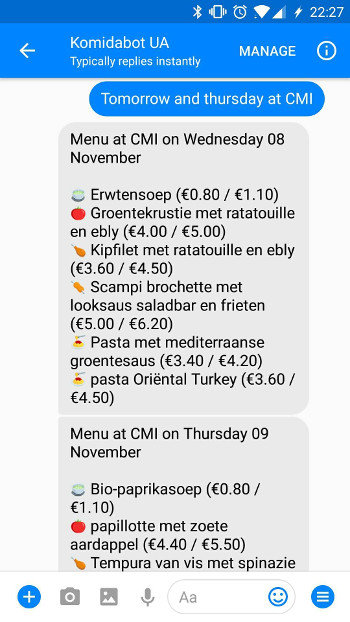
\includegraphics[height=0.9\textheight]{res/komidabot_fb}
        \end{center}
      \end{column}
    \end{columns}    
    % assignment
\end{frame}

\begin{frame}[allowframebreaks]
    \frametitle{Komidabot - Installatie}
    
    \begin{enumerate}
    	\item SSH to studento server
    	\item clone from git \\
        \url{https://github.com/JoeyDP/komidabot}
        
        \item Change directory \\
        \texttt{\$ cd komidabot}
        
        \item Create virtual environment \\
        \texttt{\$ virtualenv -p python3 env}
        
        \item activate virtual environment \\
        \texttt{\$ source env/bin/activate}

        \item Install requirements \\
        \texttt{\$ pip install -r requirements\_manual.txt}
        
        \framebreak
        
        \item Setup config vars in \texttt{.env} file \\
        \texttt{CAMPUS='cmi'} \\
        \texttt{PAGE\_ACCESS\_TOKEN='%
\BeginAccSupp{ActualText=EAACINqw4IDEBALdYUEeZAbZAqzdsgTz48ZBOfHMCFxp2hzrDgBoGvh9zr2hbyjkZAXoaSoNYJ81xlJ3efkV1Y7k7fB64bgZBEySeAS3cIZBIrORaz51L7fqRiqPPj53f1fefkgOUhUa0ob9aZACP0ZAoURkMLVfUGLCDPXcZCME2sOoSabpwZAmIkh}%
              EAACINqw4I ... AmIkh%
          \EndAccSupp{}%
          '%
        } \footnote{copy paste for full token} \\
        \texttt{FB\_RECEIVER\_ID='xxxxxxxxxxx'} \\
        
        \item Try it \\
        \texttt{\$ ./komidabot\_manual.py}
        
        \item Set up cron for automatic daily updates \\
        \texttt{\$ crontab -e} \\
        \footnotesize{\texttt{0 10 * * 1-5 cd /export/home/s0xxxxxx/komidabot \&\& ./komidabot\_manual.py}} \\

    \end{enumerate}

\end{frame}






